\section{Method}
\label{sec:method}

\begin{figure}[t]

    \centering
    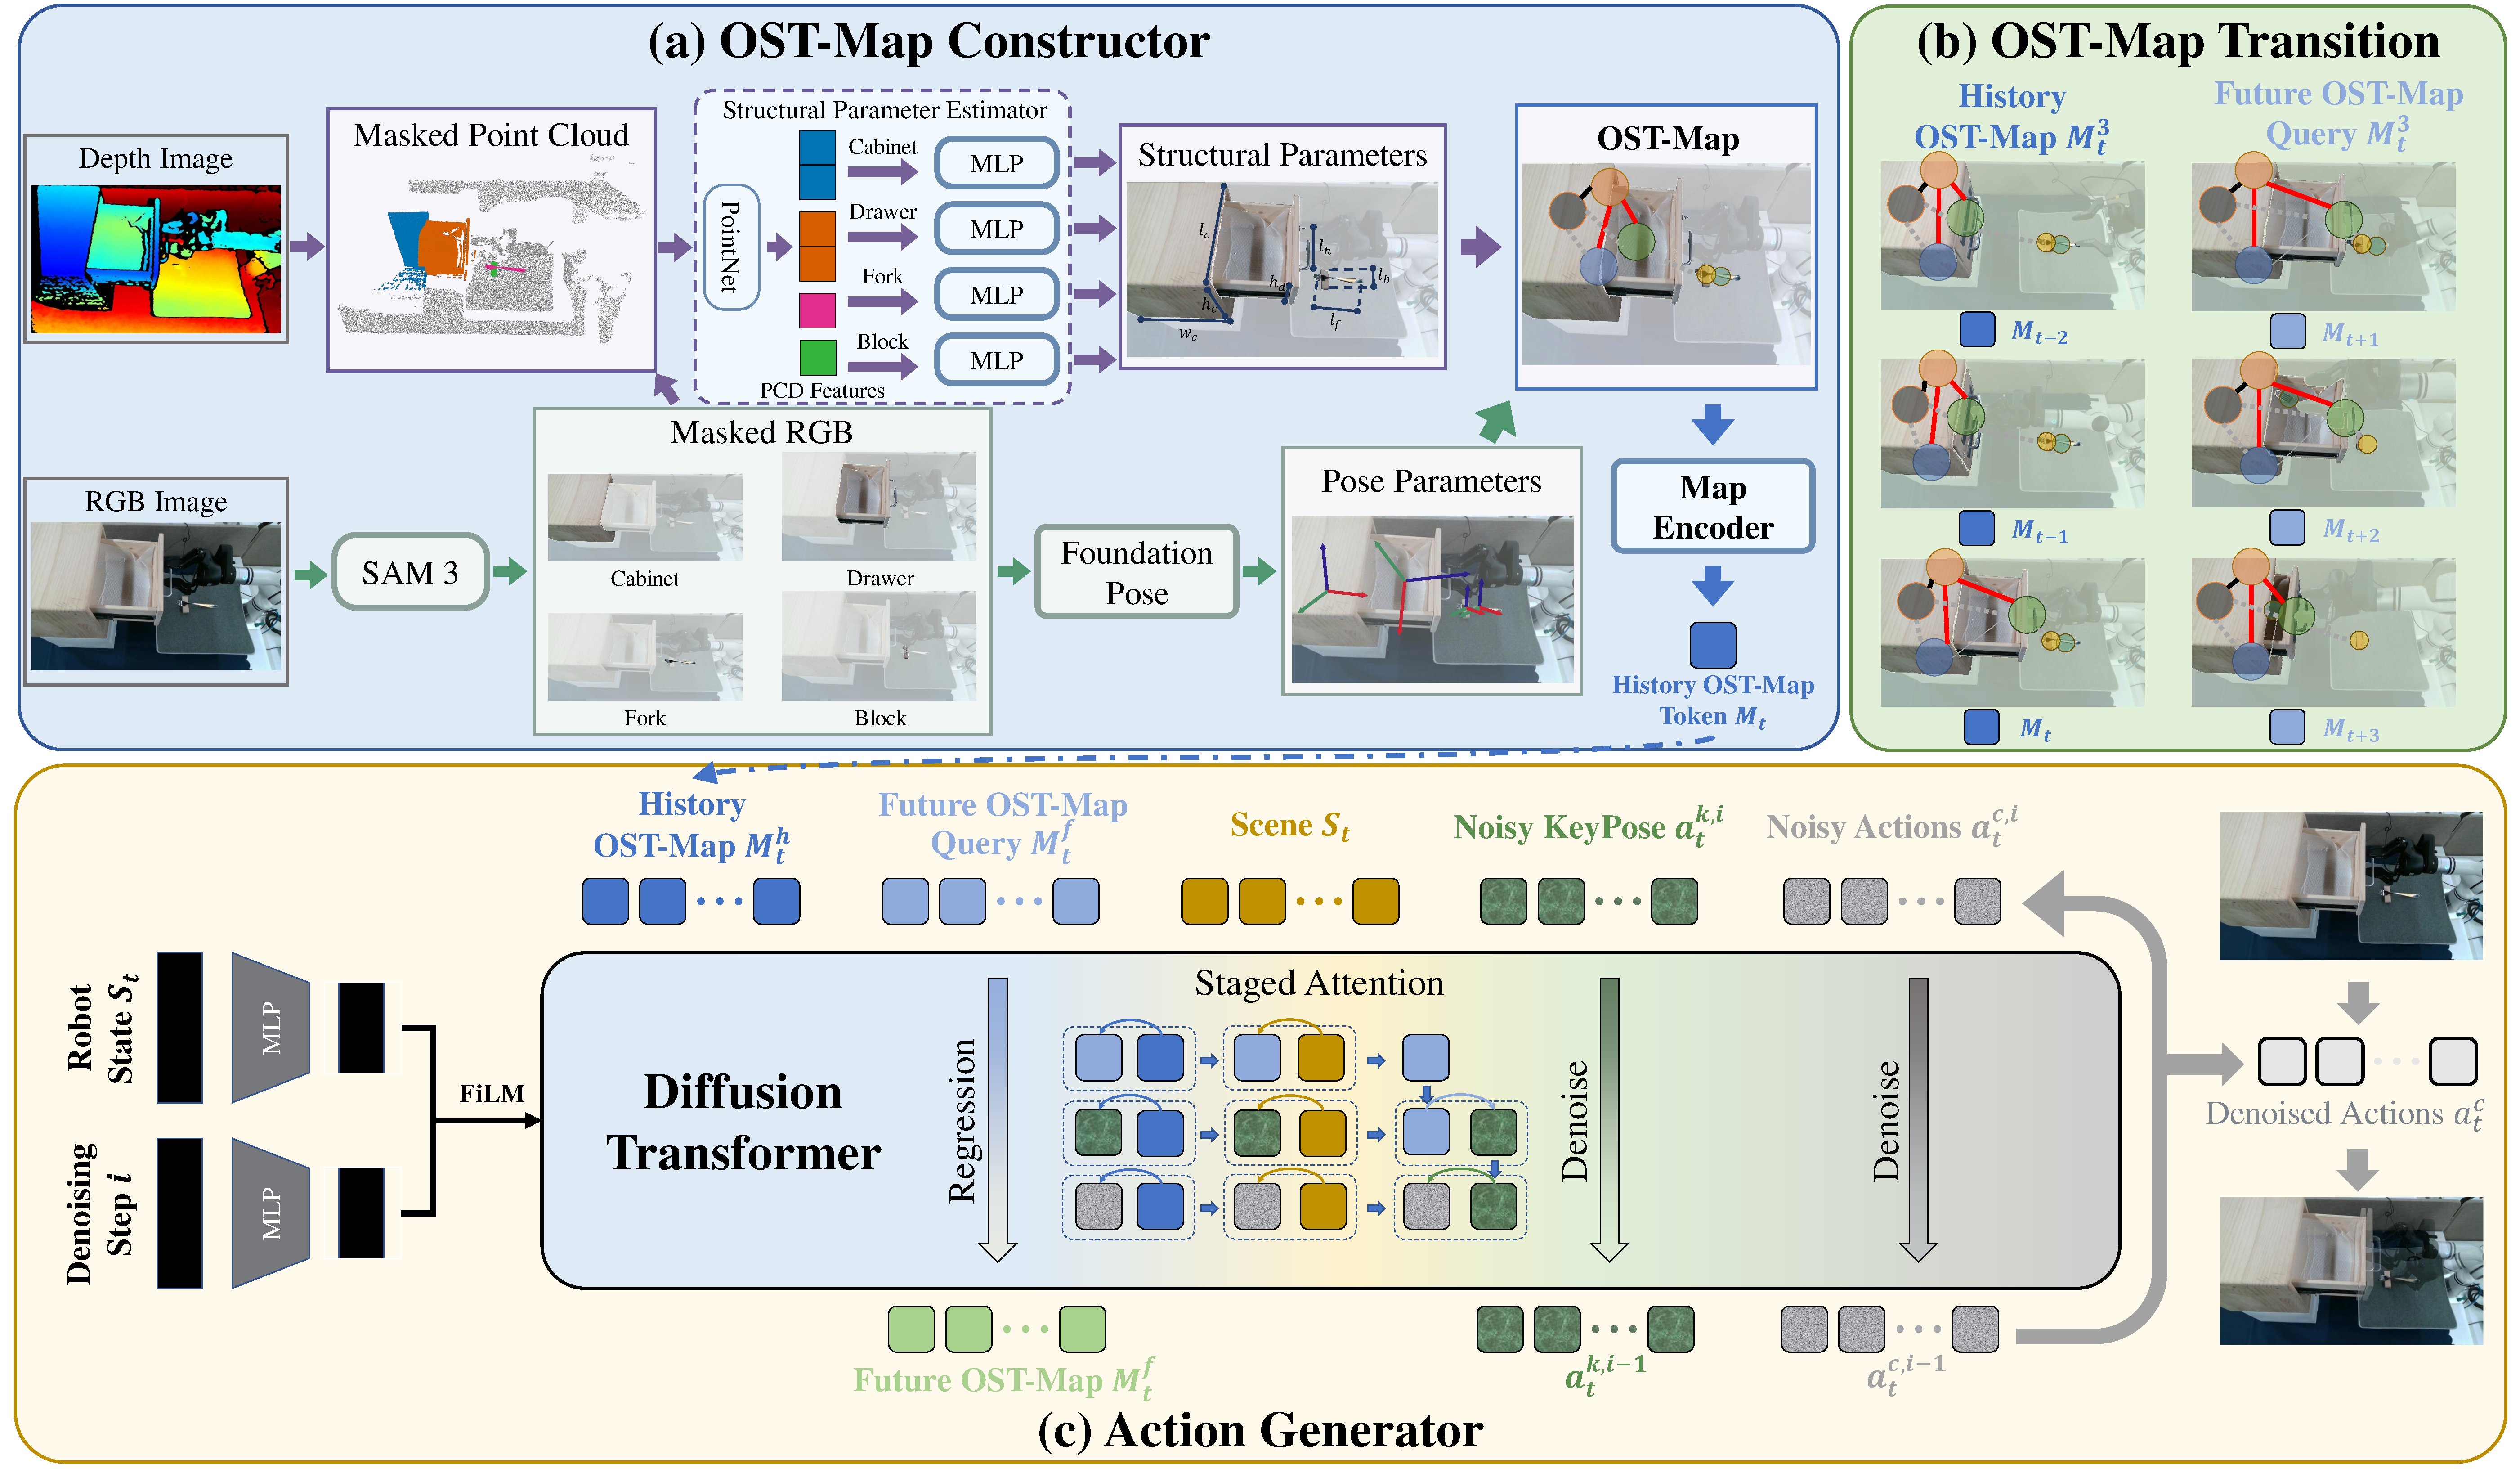
\includegraphics[width=\textwidth]{fig/2_pipeline.pdf}
    \vspace{-20pt}
    \caption{
    \textbf{Overview of OSTRA.}
    \textbf{(a) OST-Map Constructor:} RGB-D observations are converted into
    identity-consistent object-centric maps by estimating task-relevant object masks,
    structural parameters, and 6-DoF poses.
    \textbf{(b) Object-State Transition Modeling:} temporally aligned historical
    OST-Maps provide explicit object-state transition context and are used to query
    future object states.
    \textbf{(c) Transition-Guided Action Generation:} historical OST-Map tokens,
    future object-state queries, dense Semantic Field tokens, robot states, and the
    diffusion timestep are processed by OSTRA, which progressively predicts future
    object states, TCP keyposes, and continuous actions following the hierarchy
    \emph{object state $\rightarrow$ TCP subgoal $\rightarrow$ action} for
    structured multi-stage control.
    }
    \label{fig:ostra_pipeline}
    \vspace{-12pt}
\end{figure}


\subsection{Overview}
\label{sec:method_overview}

\textbf{Problem Formulation.}
We consider multi-stage robot manipulation from RGB-D observations.
At time $t$, the policy receives an observation window
$\mathcal{O}_{t}=\{(I_{\tau},D_{\tau},s_{\tau})\}_{\tau=t-T_o+1}^{t}$
and predicts an action chunk
$A_t=\{a_{t+k}\}_{k=0}^{H_a-1}$.
Rather than directly mapping the current visual observation to robot actions,
OSTRA explicitly models how task-relevant objects have evolved throughout the
observation history and which object states should be achieved next.

\textbf{Object-State Transition Modeling.}
As shown in \cref{fig:ostra_pipeline}, each RGB-D observation is converted into
an OST-Map whose identity-consistent nodes encode object semantics, structure,
affordance, and 6-DoF pose. Tracking yields aligned historical maps that expose
object-state transitions and supervise future states in the same structured
space, while a dense Semantic Field preserves local scene evidence.

\textbf{Transition-Guided Action Generation.}
Transition-Guided Attention first grounds prediction queries in historical
OST-Map tokens and then incorporates dense Semantic Field tokens. Staged Action
Generation follows the hierarchy
\emph{object state $\rightarrow$ TCP subgoal $\rightarrow$ action}:
future OST-Map keyframes condition TCP-keyframe denoising, whose representation
then conditions continuous-action generation.


\subsection{OST-Map: Object-State Transition Map}
\label{sec:ost_map}

\begin{figure}[t]
    \centering
    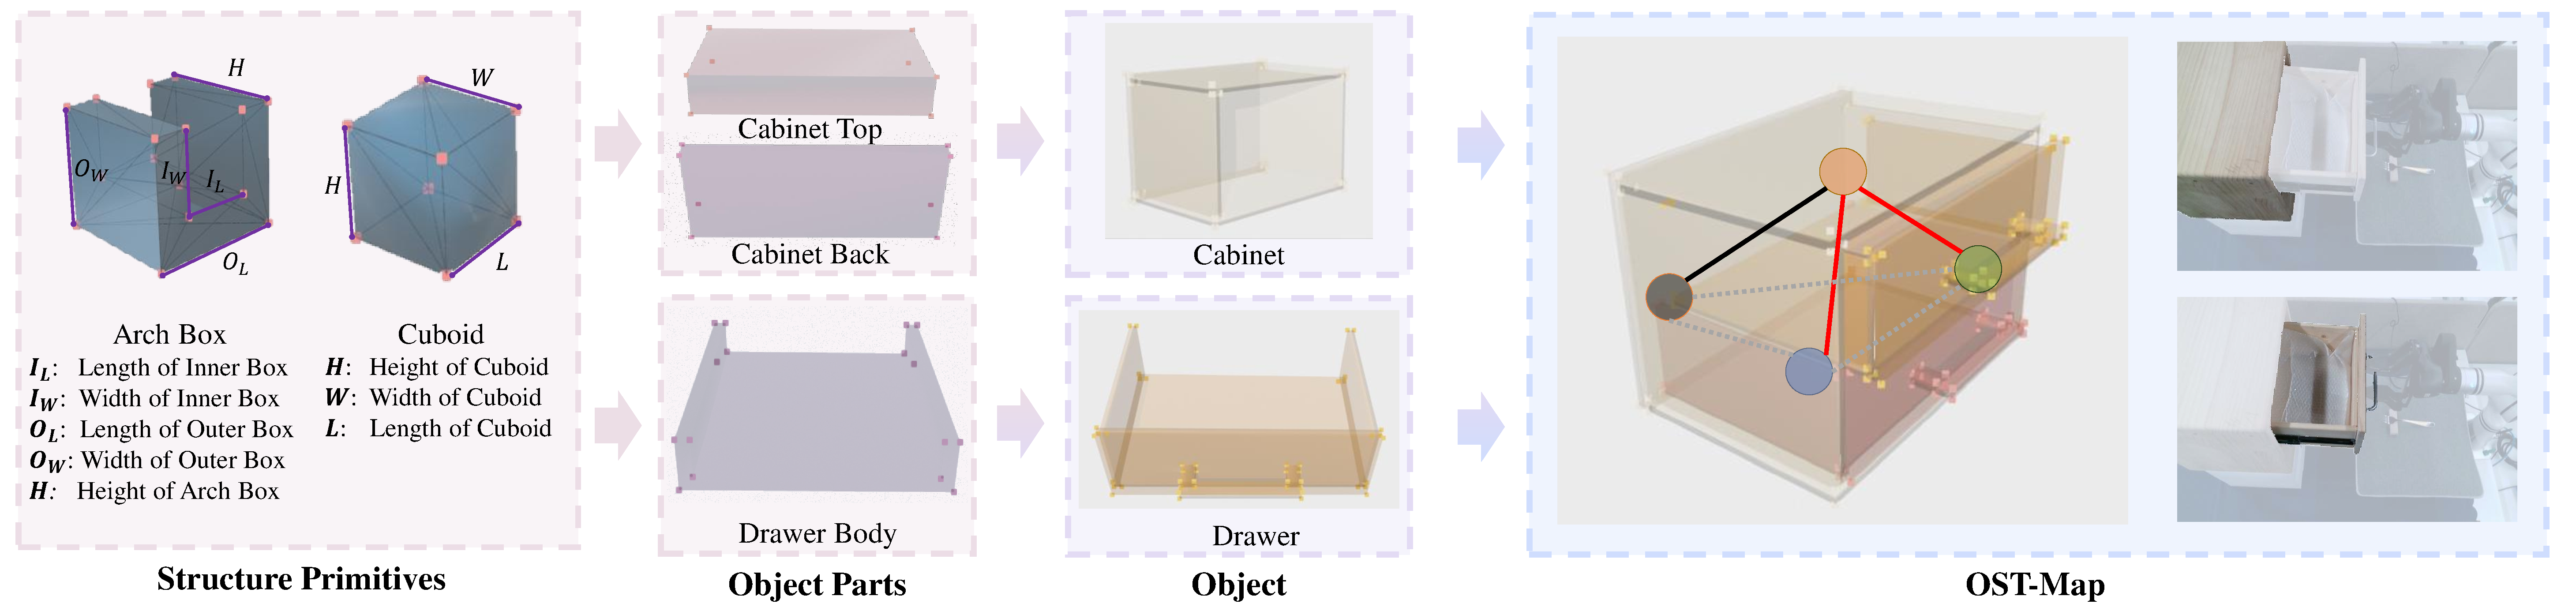
\includegraphics[width=\textwidth]{fig/3_ostmap.pdf}
    \vspace{-20pt}
    \caption{
    \textbf{Representation of OST-Map.}
    Parameterized structure primitives are composed into object parts and
    further assembled into task-relevant objects.
    Each object is represented by identity-consistent structural nodes and
    their relations, while node poses evolve with manipulation.
    The resulting OST-Map provides a compact object-centric representation of
    scene structure and object-state transitions for temporally grounded,
    multi-stage action generation.
    }
    \label{fig:ost_map}
    \vspace{-12pt}
\end{figure}

As illustrated in \cref{fig:ost_map}, OST-Map composes parameterized primitives
into object parts and identity-consistent structural nodes. Persistent node
identities preserve fine-grained structure and enable temporal tracking.

For a task with $N$ structural nodes, the OST-Map at time $t$ is defined as
an attributed graph
$\mathcal{M}_t=(\mathcal{V}_t,\mathcal{E}_t)$.
Each node $v_{t,i}\in\mathcal{V}_t$ is represented as
\begin{equation}
    v_{t,i}
    =
    \bigl(
    c_i,\mathcal{P}_i,\mathcal{A}_i,p_{t,i},q_{t,i}
    \bigr),
    \label{eq:ost_node}
\end{equation}
where $c_i$ denotes its semantic identity,
$\mathcal{P}_i$ and $\mathcal{A}_i$ denote its structural and affordance point
sets, and
$(p_{t,i},q_{t,i})\in\mathbb{R}^{3}\times\mathbb{S}^{3}$
denotes its 6-DoF pose.
Semantic identity and local structural attributes remain fixed within an
episode, while pose evolves with the object state.

Each edge $e_{t,ij}\in\mathcal{E}_t$ stores its relation type, parameters,
reference anchors, and relative pose. Free-relation edges connect pairs without
task-specific relations. The sequence $\mathcal{M}_{t-T_o+1:t}$ captures
object-state evolution in an identity-aligned space.


\subsection{OSTRA: Object-State Transition Reasoning Architecture}
\label{sec:ostra}

\textbf{OST-Map Construction and Transition Targets.}
As shown in \cref{fig:ostra_pipeline}(a), OSTRA first constructs an OST-Map
from each RGB-D observation. SAM 3~\citep{sam3} segments prompted task objects,
FoundationPose~\citep{foundationposewen2024} registers and tracks their 6-DoF
poses, and PointNet~\citep{Qi2017PointNet} with object-specific MLP heads
estimates structural parameters from masked point clouds, producing a
temporally aligned map sequence.

Historical OST-Maps encode observed transitions. During training, the
structural-node positions at the next $H_k$ task keyframes define future-state
targets, 
\begin{equation}
    Y_t^{M}
    =
    \{p^{\star}_{t,h,i}\}_{h=1,i=1}^{H_k,N}.
    \label{eq:future_map_target}
\end{equation}
paired with TCP keyframes $Y_t^{E}$ and action chunk $A_t$. Future observations
provide training-only supervision, while the shared OST-Map space supplies
identity-aligned transition targets.


\textbf{Multimodal Context Encoding.}
OSTRA combines a sparse OST-Map with a dense Semantic Field. Depth points
$X_t=\{x_{t,j}\}_{j=1}^{P}$ are paired with image-aligned pretrained DINO
features $d_{t,j}$. PointNet++ encodes
$\operatorname{concat}(x_{t,j},d_{t,j})$ into dense tokens
$F_t^{S}$ for cross-attention and downsampled tokens $\bar{F}_t^{S}$ for compact
planning context.

For each historical map, node embeddings combine PointNet features of
$\mathcal{P}_i$ and $\mathcal{A}_i$ with semantic, pose, temporal, and identity
embeddings. Edge embeddings encode relation attributes and relative pose. A
graph transformer produces coordinate-aware map tokens $F_t^{M}$. Map and scene
tokens retain 3D coordinates for relative spatial attention. Robot state and
diffusion timestep condition prediction blocks through adaptive normalization.


\textbf{Transition-Guided Attention.}
A central challenge is the large imbalance between the sparse OST-Map tokens
and the dense Semantic Field tokens.
Directly mixing them in a single attention context can weaken the structured
transition cues carried by the OST-Map.
OSTRA therefore introduces \emph{Transition-Guided Attention}, in which each
prediction query first attends to historical OST-Map tokens and subsequently
to the dense Semantic Field:
\begin{equation}
    \widetilde{Z}
    =
    \operatorname{CA}(Z,F^{M}),
    \qquad
    Z^{+}
    =
    \operatorname{CA}(\widetilde{Z},F^{S}),
    \label{eq:tga}
\end{equation}
where $\operatorname{CA}$ denotes cross-attention.
Cross-attention uses relative 3D rotary encodings computed from query and
context coordinates.

For future object-state prediction, queries repeat the latest structural-node
coordinates over the next $H_k$ keyframes
and augmenting them with learned keyframe-time and node-identity embeddings.
TCP and action queries come from their noisy diffusion variables. The map-first
order preserves transition grounding before introducing denser visual context.

\begin{table}[t]
    \vspace{-10pt}
    \centering
    \caption{\textbf{Summary of the main simulation results.}
    We report average task success rate (\%) on each benchmark.
    Full per-task results are in Appendix~\ref{app:full_sim_results}.
    \textbf{Bold} and \underline{underlining} denote the best and second-best
    results, respectively, under the benchmark-specific evaluation protocols.}
    \label{tab:main_results_summary}
    \vspace{2pt}
    \small
    \setlength{\tabcolsep}{6pt}
    \begin{adjustbox}{max width=\textwidth}
    \begin{tabular}{lc|lc|lc}
        \toprule
        \rowcolor{tablehead}
        \multicolumn{2}{c|}{RLBench2~\citep{James2020RLBench} (7 tasks)} &
        \multicolumn{2}{c|}{ManiSkill~\citep{Gu2023ManiSkill2} (6 tasks)} &
        \multicolumn{2}{c}{LIBERO~\citep{liu2023libero} (40 tasks)} \\
        \rowcolor{tablehead}
        Method & Mean S.R. (\%) & Method & Mean S.R. (\%) & Method & Mean S.R. (\%) \\
        \midrule
        ACT~\citep{Zhao2023Learning} & 15.5 &
        ACT~\citep{Zhao2023Learning} & 21.3 &
        ACT~\citep{Zhao2023Learning} & 67.7 \\
        DP3~\citep{Ze2024DP3} & 26.0 &
        Diffusion Policy~\citep{chi2024diffusionpolicy} & 26.8 &
        GROOT~\citep{zhu2023learning} & 66.2 \\
        3D Diffuser Actor~\citep{ke2024diffuseractor} & 64.7 &
        DP3~\citep{Ze2024DP3} & 53.8 &
        Diffusion Policy~\citep{chi2024diffusionpolicy} & 72.4 \\
        PerAct$^2$~\citep{shridhar2022peract} & 40.0 &
        3D Diffuser Actor~\citep{ke2024diffuseractor} & 51.5 &
        BAKU~\citep{Haldar2025BAKU} & 93.0 \\
        PPI~\citep{Yang2025PPI} & 80.8 &
        \underline{PPI~\citep{Yang2025PPI}} & \underline{56.8} &
        MDT~\citep{reuss2024multimodal} & 76.1 \\
        Diffusion Policy~\citep{chi2024diffusionpolicy} & 42.6 &
        BAKU~\citep{Haldar2025BAKU} & 43.0 &
        DP3~\citep{Ze2024DP3} & 73.0 \\
        \underline{SAM2Act+~\citep{Fang2025SAM2Act}} & \underline{84.5} &
        FlowPolicy~\citep{zhang2024flowpolicy} & 39.5 &
        UWM~\citep{Zhu2025UWM} & 91.8 \\
        GROOT~\citep{zhu2023learning} & 45.2 &
        SPOT~\citep{Hsu2025SPOT} & 47.5 &
        \underline{MemoryVLA~\citep{shi2025memoryvla}} & \underline{96.7} \\
        SPOT~\citep{Hsu2025SPOT} & 82.3 &
        Im2Flow2Act~\citep{xu2024im2flow2act} & 45.7 &
        BPP~\citep{Mark2026BPP} & 90.9 \\
        \rowcolor{tablehead}
        \textbf{OSTRA (Ours)} & \textbf{89.8} &
        \textbf{OSTRA (Ours)} & \textbf{74.5} &
        \textbf{OSTRA (Ours)} & \textbf{97.4} \\
        \bottomrule
    \end{tabular}
    \end{adjustbox}
    \vspace{-8pt}
\end{table}


\begin{algorithm}[h]
\caption{Staged Action Generation in OSTRA}
\label{alg:ostra_generation}
\begin{algorithmic}[1]
\REQUIRE Map context $F^M$, scene context $F^S$, robot state $s_t$
\ENSURE Action chunk $\widehat{A}_t$

\STATE Construct future object queries $Z^M$
\STATE Initialize $Y^{E,N},A^N\sim\mathcal{N}(0,I)$

\FOR{$n=N,\ldots,1$}
    \STATE $P^M,\widehat{Y}^M_n
    \leftarrow \textsc{ObjectStage}(Z^M,F^M,F^S,s_t,n)$

    \STATE $P^E,\widehat{\epsilon}^E_n
    \leftarrow \textsc{TCPStage}(Y^{E,n},F^M,F^S,\operatorname{sg}(P^M),s_t,n)$

    \STATE $P^A,\widehat{\epsilon}^A_n,\widehat{G}_n
    \leftarrow \textsc{ActionGenerator}(A^n,F^M,F^S,\operatorname{sg}(P^E),s_t,n)$

    \STATE $Y^{E,n-1}
    \leftarrow \textsc{Denoise}(Y^{E,n},\widehat{\epsilon}^E_n,n)$

    \STATE $A^{n-1}
    \leftarrow \textsc{Denoise}(A^n,\widehat{\epsilon}^A_n,n)$
\ENDFOR

\RETURN $A^0$ with predicted gripper states
\end{algorithmic}
\end{algorithm}
\vspace{-8pt}

\textbf{Staged Action Generation.}
As illustrated in \cref{fig:ostra_pipeline}(c), OSTRA translates
object-state transitions into executable robot motion through the hierarchy
\emph{object state $\rightarrow$ TCP subgoal $\rightarrow$ action}.
At each diffusion step, future-object queries yield an object plan $P^{M}$ and
predicted states $\widehat{Y}^{M}$. Noisy TCP queries then combine ordered
map-to-scene attention with $\operatorname{sg}(P^{M})$ to produce a TCP plan
$P^{E}$ and TCP-noise estimate. Finally, the Action Generator conditions noisy
action queries on $\operatorname{sg}(P^{E})$ to predict action noise and
gripper openness. TCP
keyframes and actions are progressively denoised from Gaussian noise, whereas
future object states are re-predicted at every step. Position and rotation use
separate schedules. Algorithm~\ref{alg:ostra_generation} summarizes the procedure.


\textbf{Training Objective and Inference.}
OSTRA is trained with direct supervision at all three levels of the hierarchy.
The objective combines future object-state prediction, TCP diffusion, action
diffusion, and gripper supervision:
\begin{equation}
\begin{split}
    \mathcal{L} ={}&
    \lambda_M
    \lVert\widehat{Y}^{M}-Y^{M}\rVert_1
    +
    \lambda_E
    \lVert\widehat{\epsilon}_{E}-\epsilon_E\rVert_1 \\
    &+
    \lambda_A
    \lVert\widehat{\epsilon}_{A}-\epsilon_A\rVert_1
    +
    \lambda_G
    \lVert\widehat{G}-G\rVert_1 .
\end{split}
\label{eq:total_loss}
\end{equation}
The terms supervise object evolution, TCP subgoals, continuous control, and
gripper state. Stop-gradient requires each stage to satisfy its own target.

At inference, map and field contexts are encoded once per replanning step. Each
reverse step executes Algorithm~\ref{alg:ostra_generation}. The policy
executes the first predicted actions and replans from the updated history.
